\documentclass[10pt]{article}
\usepackage[polish]{babel}
\usepackage[utf8]{inputenc}
\usepackage[T1]{fontenc}
\usepackage{amsmath}
\usepackage{amsfonts}
\usepackage{amssymb}
\usepackage[version=4]{mhchem}
\usepackage{stmaryrd}
\usepackage{graphicx}
\usepackage[export]{adjustbox}
\graphicspath{ {./images/} }

\title{X Konkurs matematyczny St@ś }

\author{}
\date{}


\begin{document}
\maketitle
XIV LO im. Stanisława Staszica\\
2 czerwca 2010 roku

\section*{klasa VI}
Na rozwiqzanie poniższych zadań masz 90 minut.\\
Kolejność rozwiqzywania tych zadań jest dowolna.\\
Wszystkie zadania sa jednakowo punktowane.\\
Maksymalnq liczbę punktów może uzyskać jedynie pelne rozwiqzanie, z uzasadnieniem i odpowiedzia.\\
Uzywanie korektora i korzystanie z kalkulatora jest niedozwolone.

\section*{Zadanie 1.}
Dany jest trapez równoramienny \(A B C D\) (jak na rysunku). Odcinek \(B E\) jest prostopadły do ramienia \(A D\). Dane są długości odcinków: \(|B F|=3,|E F|=|E D|=1\). Oblicz długość przekątnej \(A C\).\\
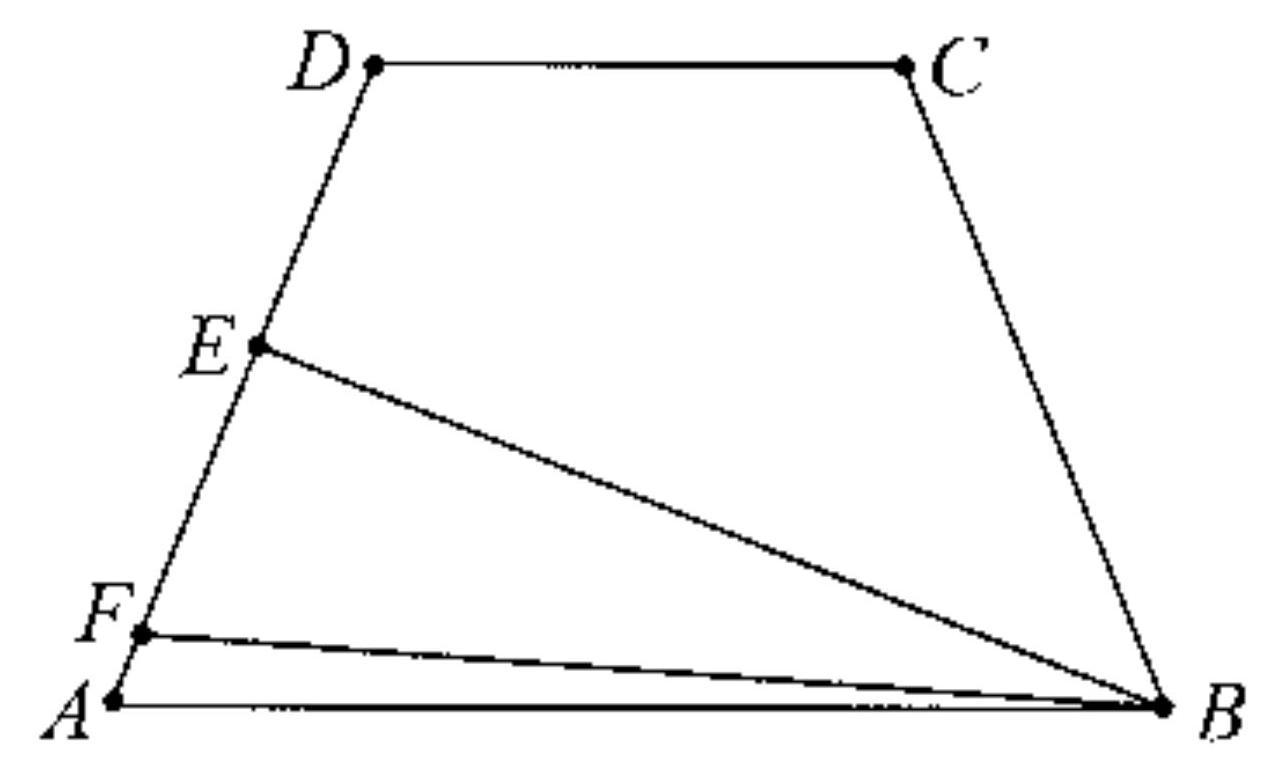
\includegraphics[max width=\textwidth, center]{2024_11_21_419bcdc1680818eb8347g-1}

\section*{Zadanie 2.}
W pewnej liczbie trzycyfrowej zamieniono cyfrę dziesiątek z cyfrą jedności, tworząc w ten sposób nową liczbę trzycyfrową. Suma obu liczb jest równa 1187. Wyznacz te liczby.

\section*{Zadanie 3.}
Dzielna i dzielnik są liczbami dwucyfrowymi, a iloraz i reszta są równymi liczbami jednocyfrowymi. Dzielnik jest równy iloczynowi ilorazu i reszty. Wyznacz dzielna.

\section*{Zadanie 4.}
Czy w graniastosłupie suma liczby ścian, liczby wierzchołków i liczby krawędzi może być równa 2010?

\section*{Zadanie 5.}
Napisz siedem różnych liczb naturalnych spełniających jednocześnie dwa następujące warunki:

\begin{enumerate}
  \item żadna z tych liczb nie dzieli się przez 3 ,
  \item suma dowolnych trzech spośród tych liczb dzieli się przez 3.
\end{enumerate}

\end{document}